\documentclass{beamer}
% Use DS9 global theme
\usepackage{../../../shared/templates/ds9_theme}

% Additional packages
\usepackage{booktabs}
\setbeamercolor{frametitle}{bg=ds9blue,fg=white}
\setbeamercolor{block title}{bg=ds9blue,fg=white}
\setbeamercolor{block body}{bg=ds9grey!20,fg=black}


% Title page configuration
\title[Place-Based Knowledge]{Indigenous Perspectives in STEAM}
\subtitle{Integrating Place-Based Knowledge with Scientific Principles}
\author[Mr. Gullo]{Mr. Gullo}
\institute{Physics Department}
\date[March 2025]{March, 2025}

% Start of document
\begin{document}

% Title page
\begin{frame}
    \titlepage
\end{frame}

\section{Learning Objectives}

\begin{frame}{Learning Objectives}
    \begin{block}{By the end of this presentation, you will be able to:}
        \begin{itemize}
            \item Describe the relationship between place-based knowledge and scientific understanding
            \item Identify key elements of Indigenous physics perspectives
            \item Recognize parallel concepts between traditional knowledge and modern physics
            \item Apply diverse knowledge systems to solve physics problems
            \item Evaluate how Indigenous perspectives can enhance scientific inquiry
        \end{itemize}
    \end{block}
\end{frame}



\section{Background on Place-Based Knowledge}

\begin{frame}{Place-Based Knowledge: Foundations}
    \begin{columns}
        \column{0.6\textwidth}
        \begin{itemize}
            \item Knowledge deeply connected to specific locations
            \item Understanding derived from direct experience with environments
            \item Knowledge passed through generations of observation
            \item Emphasis on relationships between phenomena
            \item Context-dependent rather than abstract
        \end{itemize}
        
        \column{0.4\textwidth}
        \begin{figure}
            \centering
            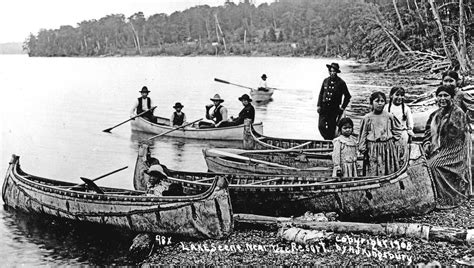
\includegraphics[width=0.75\linewidth]{cs12-history-indigenous-people-canoes.jpg}
        \end{figure}
    \end{columns}
    
    \begin{alertblock}{Key Insight}
        Place-based knowledge recognizes that understanding is embedded in specific contexts rather than universal abstractions.
    \end{alertblock}
\end{frame}

\section{Indigenous Physics Concepts}

\begin{frame}{Relational Understanding in STEAM}
    \begin{block}{Western Approach}
        \begin{itemize}
            \item Isolates variables for study prediction
            \item Reduces systems to fundamental parts
            \item Seeks universal laws
        \end{itemize}
    \end{block}
    
    \begin{block}{Indigenous Approach}
        \begin{itemize}
            \item Emphasizes interconnectedness of phenomena
            \item Studies relationships between elements
            \item Recognizes context-dependent variations
        \end{itemize}
    \end{block}
    
    \begin{exampleblock}{Example Application}
        Understanding wave phenomena through observing interactions in natural water systems rather than through isolated wave equations.
    \end{exampleblock}
\end{frame}

\begin{frame}{Observational Expertise}
    \begin{itemize}
        \item Knowledge built through generations of careful observation
        \item Detailed understanding of patterns and cycles
        \item Recognition of subtle environmental indicators
        \item Correlation of multiple phenomena simultaneously
    \end{itemize}
    
    \begin{alertblock}{Connection to Scientific Method}
        Both Indigenous knowledge and modern science value observation as a primary tool, but differ in recording methods and time scales.
    \end{alertblock}
    
   \begin{figure}
       \centering
       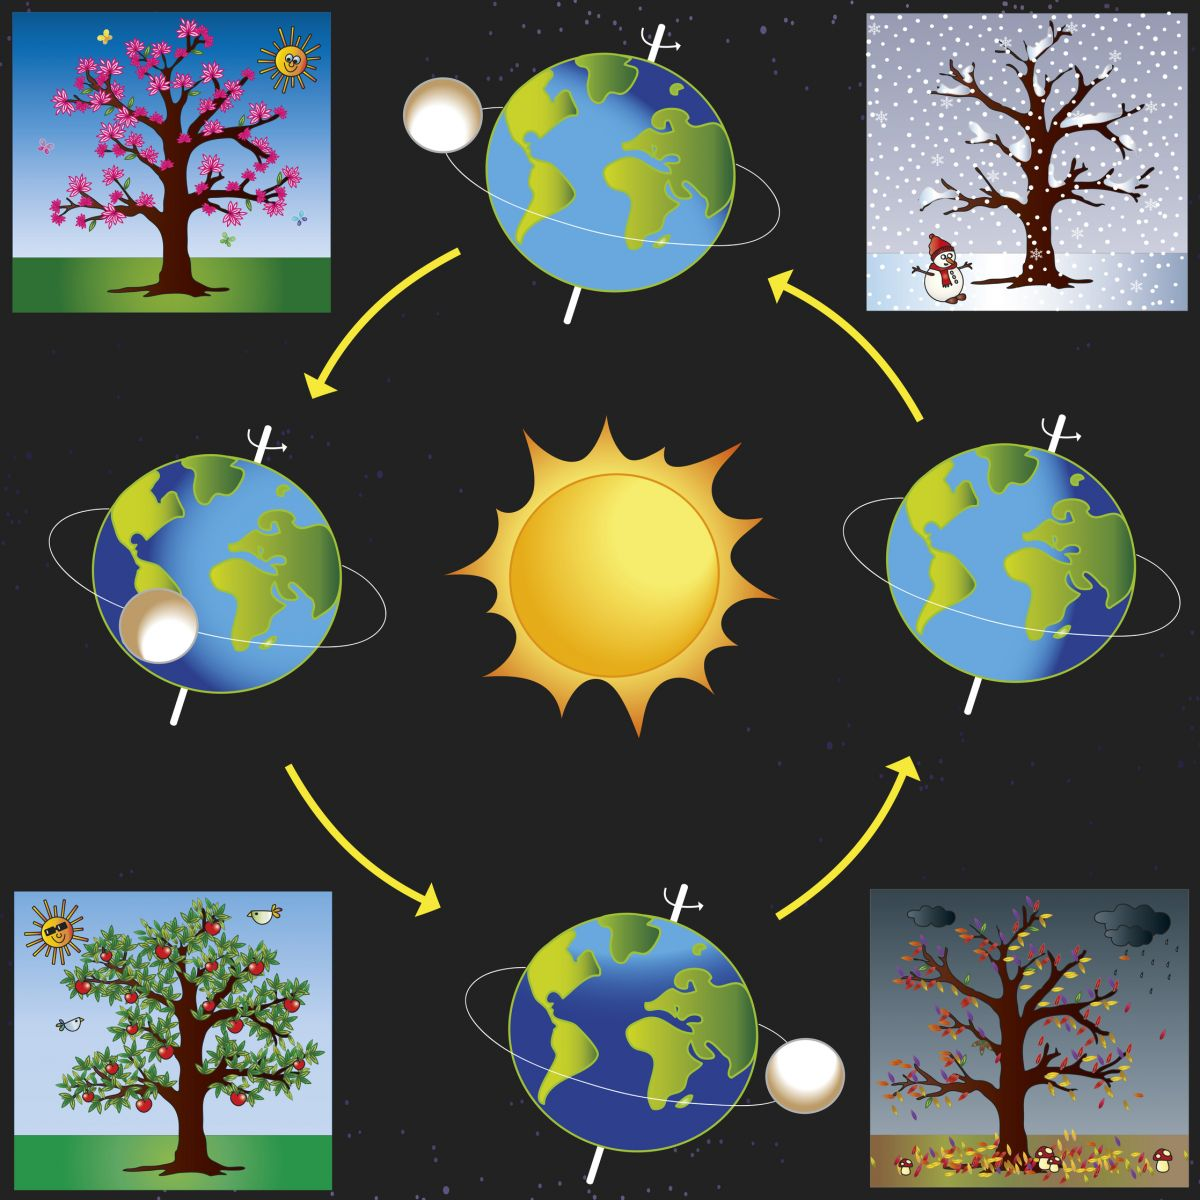
\includegraphics[width=0.3\linewidth]{cs12-earth-seasons-diagram.jpg}
   \end{figure}
\end{frame}

\begin{frame}{Holistic Approaches to Physical Phenomena}
    \begin{columns}
        \column{0.5\textwidth}
        \textbf{Western Scientific Approach}
        \begin{itemize}
            \item Studies phenomena in isolation
            \item Controls variables
            \item Seeks objective measurement
            \item Prioritizes quantitative data
        \end{itemize}
        
        \column{0.5\textwidth}
        \textbf{Indigenous Approach}
        \begin{itemize}
            \item Examines phenomena in context
            \item Observes interrelationships
            \item Incorporates multiple perspectives
            \item Values qualitative observations
        \end{itemize}
    \end{columns}
    
    \begin{block}{Complementary Nature}
        These approaches can be seen as complementary rather than contradictory, offering different insights into the same phenomena.
    \end{block}
\end{frame}

\begin{frame}{Astronomical Knowledge}
    \begin{itemize}
        \item Many Indigenous communities developed sophisticated celestial understanding
        \item Star positions used for navigation, timekeeping, and seasonal planning
        \item Recognition of planetary movements and cycles
        \item Correlation between celestial events and Earth-based phenomena
        \item Integration of astronomical knowledge into cultural practices
    \end{itemize}
    
    \begin{exampleblock}{Example: Celestial Navigation}
        Pacific Islander wayfinding techniques incorporate detailed knowledge of star positions, ocean currents, and wave patterns to navigate vast distances.
    \end{exampleblock}
    
\end{frame}

\begin{frame}
\begin{figure}
    \centering
    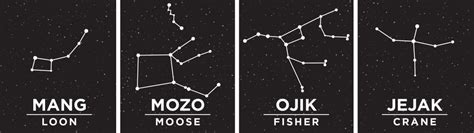
\includegraphics[width=0.95\linewidth]{cs12-astronomy-indigenous-constellations.png}
\end{figure}
\end{frame}
\begin{frame}{
}
    
\begin{figure}
    \centering
    \includegraphics[width=0.95\linewidth]{cs12-place-maori_astronomy.png}
\end{figure}
\end{frame}
\begin{frame}
\begin{figure}
    \centering
    \includegraphics[width=0.95\linewidth]{../images/cs12-place-maori_astronomy.png}
\end{figure}
\end{frame}


\begin{frame}{Sustainable Technologies}
    \begin{block}{Physics Principles in Traditional Technologies}
        \begin{itemize}
            \item Canoe design: Hydrodynamics, buoyancy, stability
            \item Architecture: Thermodynamics, material properties, structural mechanics
            \item Hunting tools: Projectile motion, energy transfer, aerodynamics
            \item Navigation techniques: Astronomy, wave dynamics, wind patterns
            \item Agricultural practices: Soil physics, hydrology, seasonal energy cycles
        \end{itemize}
    \end{block}
    
    \begin{alertblock}{Key Insight}
        Indigenous technologies often optimize for sustainability rather than maximizing immediate output.
    \end{alertblock}
\end{frame}

\section{Indigenous Computer Science Connections}

\begin{frame}{Pattern Recognition and Algorithmic Thinking}
   
        \begin{itemize}
            \item Indigenous beadwork, weaving, and quillwork incorporate complex patterns
            \item These patterns follow systematic algorithms
            \item Pattern recognition central to both traditions
            \item Both require precise sequence of operations
            \item Both involve error detection and correction
        \end{itemize}
    
    \begin{exampleblock}{Example Connection}
        The iterative patterns in traditional weaving can be represented as recursive algorithms in computer science.
    \end{exampleblock}
\end{frame}

\begin{frame}{Data Stewardship and Ethics}
    \begin{block}{Indigenous Approaches to Knowledge Management}
        \begin{itemize}
            \item Knowledge access determined by appropriate use and relationship
            \item Consideration of impacts across generations
            \item Protocols for information sharing and protection
            \item Recognition of knowledge as living rather than static
            \item Emphasis on responsible use of information
        \end{itemize}
    \end{block}
    
    \begin{block}{Relevance to Modern Data Ethics}
        These principles offer valuable perspectives for addressing contemporary challenges in data privacy, ownership, and algorithmic bias.
    \end{block}
\end{frame}

\begin{frame}{Systems Thinking}
    \begin{itemize}
        \item Understanding the world as interconnected systems
        \item Recognition of feedback loops and emergent properties
        \item Awareness of cascading effects across system boundaries
        \item Consideration of multiple timescales simultaneously
        \item Focus on relationships between components
    \end{itemize}
    
    \begin{alertblock}{Connection to Computer Science}
        Systems thinking provides valuable perspectives for complex systems design, network architecture, and software ecosystems.
    \end{alertblock}
    
\end{frame}

\section{Integrating Knowledge Systems}

\begin{frame}{Complementary Approaches}
    \begin{columns}
        \column{0.5\textwidth}
        \textbf{Strengths of Western Science}
        \begin{itemize}
            \item Precise quantitative measurement
            \item Controlled experimentation
            \item Mathematical modeling
            \item Replicability across contexts
            \item Rapid hypothesis testing
        \end{itemize}
        
        \column{0.5\textwidth}
        \textbf{Strengths of Indigenous Knowledge}
        \begin{itemize}
            \item Long-term observation
            \item Contextual understanding
            \item Holistic perspectives
            \item Ethical frameworks
            \item Practical applications
        \end{itemize}
    \end{columns}
    
    \begin{block}{Integration Benefits}
        Combining these approaches can lead to more comprehensive understanding and more effective, sustainable solutions.
    \end{block}
\end{frame}

\begin{frame}{Research Opportunities}
    \begin{block}{Potential Research Projects}
        \begin{itemize}
            \item Comparing traditional weather prediction methods with meteorological models
            \item Analyzing the physics principles in traditional technologies
            \item Developing educational approaches that integrate multiple knowledge systems
            \item Examining how traditional ecological knowledge can inform climate science
            \item Exploring how Indigenous astronomy correlates with modern astrophysics
        \end{itemize}
    \end{block}
    
    \begin{alertblock}{Methodological Considerations}
        Effective research requires respectful collaboration, recognition of knowledge ownership, and appropriate protocols for information sharing.
    \end{alertblock}
\end{frame}

\section{Summary}

\begin{frame}{Key Takeaways}
    \begin{block}{Summary Points}
        \begin{itemize}
            \item Indigenous knowledge systems offer valuable perspectives on physical phenomena
            \item Place-based knowledge emphasizes context and relationships
            \item Traditional technologies demonstrate sophisticated understanding of physics principles
            \item Indigenous and Western approaches can complement each other
            \item Integrating diverse knowledge systems can enrich science education and research
        \end{itemize}
    \end{block}
    
    \begin{alertblock}{Call to Action}
        As STEAM students, consider how incorporating diverse perspectives might enhance your understanding of natural phenomena and lead to more creative problem-solving.
    \end{alertblock}
\end{frame}

\begin{frame}{Questions for Discussion}
    \begin{enumerate}
        \item How might observation-based knowledge complement equation-based knowledge?
        \item What advantages might come from considering physical phenomena in their broader context?
        \item How could traditional technological solutions inform modern sustainability challenges?
        \item What ethical considerations from Indigenous knowledge systems might benefit modern scientific practice?
        \item How can we respectfully integrate diverse knowledge systems while acknowledging their distinct origins and purposes?
    \end{enumerate}
\end{frame}

\begin{frame}
    \begin{center}
        \Huge\textcolor{ds9blue}{Thank You}
        
        \vspace{1cm}
        
        \large Questions and Discussion
    \end{center}
\end{frame}

\end{document}